\section{Introduction}
\label{sec:intro}

Simultaneous speech-to-speech translation (SimulS2ST) must start speaking the translation before the speaker has finished.
Recent speech language models such as Qwen3-Omni~\citep{xu2025qwen3omni} translate speech accurately when they hear the whole utterance~\citep{uniss2025}.
The most direct way to run them simultaneously is re-translation~\citep{arivazhagan2020retranslation,machacek2023turning}: every $\Delta$ seconds the model re-drafts the full translation from all audio heard so far, and a commit rule decides how much of the draft is handed to the speech synthesizer.
Committed speech cannot be withdrawn.
The commit rule therefore carries the whole quality--latency trade-off, while the drafter itself stays unchanged.

The default rule is local agreement~\citep{liu2020low,polak2022cuni}.
It commits the longest common prefix of the two most recent drafts.
Agreement is a weak proxy for correctness.
A full-sentence model completes partial input with a plausible guess, and two consecutive guesses often coincide, so local agreement commits anticipations that a later read overturns.
Adding a second check fixes this but delays speech.
For example, the draft from an enhanced copy of the audio may also be required to agree; in our experiments this raises ASR-BLEU by 0.9--1.2 points and postpones speech by 0.36--0.37\,s.
Hard combinations of checks move along one quality--latency curve without pushing it outward.

We argue that the right object is not a rule over checks but a belief over a latent state.
At every read, each draft position is either \emph{settled}, meaning its content will not change any more, or still \emph{unsettled}.
Agreement across reads, agreement across acoustic views, a verifier's judgement that the speech supports the text, and the drafter's confidence are noisy certificates of that state.
Their reliability depends on the acoustics: cross-view disagreement is harmless when the enhancer works hard, but informative on clean speech.
A hidden semi-Markov model (HSMM)~\citep{yu2010hsmm} whose duration prior and emissions are driven by acoustic inputs~\citep{bengio1995iohmm} fuses these certificates in a principled way.
Filtering it gives the probability that each position has settled.
The commit rule becomes a single threshold on that probability.

Two obstacles stand between this idea and a working system.
First, the latent state learned by maximum likelihood need not mean what the commit rule needs.
Trained without labels, the HSMM attaches ``settled'' to the most coherent cluster of evidence, which is ``supported by the verifier and agreed across views''.
The resulting posterior is pessimistic and badly calibrated: positions it rates below $0.02$ survive to the final translation 24--35\% of the time.
We therefore \emph{anchor} the latent state: a discriminative term trains the filtering posterior that is used online to predict whether the current prefix survives, inside the same differentiable graph as the generative likelihood.
Second, local agreement never asks whether the text is supported by what has been heard.
We add a \emph{support verifier}, a low-rank adapter on the same backbone trained only on forced-aligned references, which stops its continuation exactly where the heard speech stops supporting the translation.
Finally, a commitment can end inside a subword token, which leaves the next draft an unnatural token split; \emph{boundary healing} repairs it.

\begin{figure}[t]
  \centering
  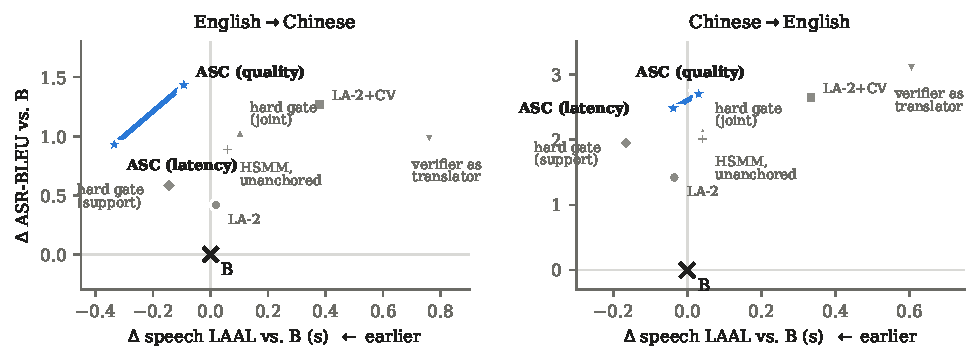
\includegraphics[width=\linewidth]{figures/frontier.pdf}
  \caption{Commit policies on one drafter relative to the local-agreement baseline B (origin), averaged over five test conditions; up-left is better.
  Rule-based combinations of certificates (grey) share one curve; \ours{} (blue; dev-selected quality and latency points) lies above it.}
  \label{fig:frontier}
\end{figure}

We call the resulting method \ours{} (\emph{Anchored Stability Commitment}).
We evaluate it on real interpreting speech~\citep{cheng2024realsi} and on broadcast-style streams under clean, in-distribution and out-of-distribution noise, in both English--Chinese directions.
One bidirectional model is used for every trained component.
\Cref{fig:frontier} summarises the outcome.
At the speech latency of the local-agreement baseline, \ours{} reaches the translation quality of the much slower cross-view system.
Our contributions are:
\begin{itemize}[leftmargin=*,itemsep=1pt,topsep=2pt]
  \item Prefix commitment as filtering of a per-unit settledness state with an input-driven HSMM over certificates whose reliability depends on the acoustics (\cref{sec:hsmm}).
  \item Anchored end-to-end training through the forward algorithm, which ties the latent state to survival and makes a single threshold the Bayes-optimal rule under homogeneous evidence (\cref{sec:anchor,sec:rule}).
  \item A speech-support verifier trained only from aligned references, and boundary healing for subword drafters (\cref{sec:cert,sec:heal}).
  \item An anatomy of the remaining latency showing that the commit layer is near its information limit (\cref{sec:anatomy}).
\end{itemize}
